\documentclass[letterpaper,10pt,titlepage]{IEEEtran}
\usepackage{lipsum}
\usepackage{graphicx}
\usepackage{amssymb}
\usepackage{amsmath}
\usepackage{amsthm}

\usepackage{alltt}
\usepackage{float}
\usepackage{color}
\usepackage{url}
\usepackage{listings}
\lstset{ 
   language=C++,                % choose the language of the code
   basicstyle=\small,        % the size of the fonts that are used for the code
   keywordstyle=\color{blue},
   stringstyle=\color{red},
   commentstyle=\color{green},
   numbers=left,                   % where to put the line-numbers
   numberstyle=\footnotesize,      % the size of the fonts that are used for the line-numbers
   stepnumber=1,                   % the step between two line-numbers. If it is 1 each line will be numbered
   numbersep=5pt,                  % how far the line-numbers are from the code
   backgroundcolor=\color{white},  % choose the background color. You must add \usepackage{color}
   showspaces=false,               % show spaces adding particular underscores
   showstringspaces=false,         % underline spaces within strings
   showtabs=false,                 % show tabs within strings adding particular underscores
   frame=single,           % adds a frame around the code
   tabsize=2,          % sets default tabsize to 2 spaces
   captionpos=b,           % sets the caption-position to bottom
   breaklines=true,        % sets automatic line breaking
   breakatwhitespace=false,    % sets if automatic breaks should only happen at whitespace
   escapeinside={\%*}{*)}          % if you want to add a comment within your code
   }
   \usepackage{balance}
   \usepackage[TABBOTCAP, tight]{subfigure}
   \usepackage{enumitem}
   \usepackage{pstricks, pst-node}

   \usepackage{geometry}
   \usepackage{longtable,hyperref}
   \geometry{textheight=8.5in, textwidth=6in, margin=0.75in}

   %\graphicspath{ /nfs/stak/students/p/palmiteh/CS461/Winter_Midterm/ }
 
   \renewcommand*\rmdefault{cmr}

   \newcommand{\cred}[1]{{\color{red}#1}}
   \newcommand{\cblue}[1]{{\color{blue}#1}}
   \newcommand{\itab}[1]{\hspace{4em}\rlap{#1}}


   \title{Midterm Progress Report}
   \author{Hailey Palmiter Scott Griffy Ryan Kitchen}
   \date{\today}

   %% The following metadata will show up in the PDF properties
   \hypersetup{
      colorlinks = true,
      urlcolor = black,
      pdfauthor = {Palmiter, Griffy, Kitchen},
      pdftitle = {Midterm Progress Report},
      pdfsubject = {CS462},
      pdfpagemode = UseNone
   }
   \begin{document}
   \begin{titlepage}
      \centering
      \vfill
      {\bfseries\Large
         Midterm Progress Report \\
         CS 462 - Senior Capstone\\
         \vskip2cm
         February 9th, 2016\\
         \vskip2cm
         The HawkEyed Crew - Group 4\\ 
         \vskip1cm
         Hailey Palmiter\\
         \vskip1cm
         Ryan Kitchen\\
         \vskip1cm
         Scott Griffy\\
    
      }
      \vfill
      \vskip2cm
      \begin{abstract}
      This document is a midterm progress report that covers a brief introduction of our senior project, our current progress, problems that have impeded our progress, and any preliminary results that have been gathered. It also describes what is left to do before all of the requirements are met for the project along with the potential for some stretch goals if time allows. This report includes a few interesting pieces of code and a description of what this code does. It is constructed using the IEEEtran style guidelines.
      \end{abstract}
      \vfill
   \end{titlepage}
   
   \onecolumn
   \tableofcontents
   \newpage
   \bigskip
   \section{Introduction}
   Our project sponsor, Rockwell Collins, currently develops and deploys their image processing architecture for airborne manned vision systems on a Field Programmable Gate Array (FPGA).  These FPGAs are not only very complex to develop on, but are also very costly and time consuming. It requires experts to integrate any new algorithms or filters into the system, which can takes weeks or months depending upon the code. The FPGAs are their only current option that meets the low power, low latency, and high bandwidth requirements they need.\\ 
\par
Our goal is to provide a proof of concept using single board computers to meet the specific requirements Rockwell Collins needs for their vision systems. This should use low cost hardware with a quick development and implementation time. Our project tests and measures the capabilities of a single board computer by delivering a multiple-stream video display based on a modular processing system. This proof of concept will result in measurable capabilities that can help Rockwell Collins determine the practicality of using single board computers for their vision systems.

   \section{Current Progress}
   \subsection{Refined Requirements Document}
   At the beginning of the term, we revised our requirements document. The revision was needed in order to refine our project with the discovery of problems/improvements. The changes were reviewed with our sponsor and agreed upon before any final changes were made. The most current requirements document was uploaded to the SharePoint as Revised\_ReqDoc on January 15th.\\ 
\par
Only a few minor things were changed, but they had a big impact on how we define our deliverable. Our client was very happy to see the revisions we made and all revisions were agreed upon. One of these changes was making sure we have two working cameras for our system and allowing us to use only the Jetson TK1 or the Jetson TX1. As we move forward we plan to rely more heavily on the TX1, but want to allow ourselves the room to be able to fall back on the TK1 if need be to complete our project. Either of these single board computers would meet the requirements of our client.
   
   \subsection{Jetson TK1}
   We have installed graphics drivers on the TK1 as well as a driver for the original PointGrey camera we were loaned by Rockwell Collins, but had a lot of difficulty working with the USB 3.0 port, due to kernel support for it being disabled. We found that the Jetson TK1's operating system had to be recompiled in order to grab full 2048x2048 pixel images from the camera. Without the recompiled kernel we were able to grab images at a lower resolution using the FlyCapture API, and could only utilize the PointGrey camera as a USB 2.0 device, not USB 3.0. Even after the recompile of the kernel we still had connection issues and display latency with the video. We quickly began to realize that development on the TK1 may not even be worth the struggle, and have moved our development process to the TX1.\\ 
\par
It would be possible to continue development on the TK1, but it does not seem to be the best option to obtain the greatest results moving forward with development. If time permits we will test our software system on the TK1 to measure its capabilities in comparison with the Jetson TX1.
   
   \subsection{Jetson TX1}
   After discovering a manufacturer error on the original TX1s, we continued development on the TK1 until the new, fully functional, TX1 arrived. This was the point when development shifted from the TK1 to the TX1.\\ 
   
   \subsubsection{Video Output}
   The first step with working with the Jetson TX1 was to get a working video output from the onboard camera, which was successful. We were able to display the image at 1080p with the option of 30 or 60 frames per second. This video stream used embedded gstreamer code to transform the image buffer generated from the camera into a Video4Linux compatible format, which is a widely compatible format with a lot of software. The image was then read with a built-in web application and displayed to the monitor. After we were able to get the video output from the PointGrey cameras working we implemented two basic edge detection functions using several of OpenCV's built-in functions to gain familiarity with the OpenCV API.\\
   
   \subsubsection{Hardware}
   Our next focus was on getting two cameras' video streams displayed to a monitor. We prioritize this before moving on to fixing the quality of the output or adding custom filters. We decided that using two USB 3.0 cameras would be the best way to progress in order to accomplish alpha release goals. But first, we had to get the USB 3.0 PointGrey camera that Rockwell Collins had supplied for us working. Once the camera was working, we were able to display the stream from the PointGrey camera on our TV. We were even able to apply some built-in filters from OpenCV. Now that we had this capability, we discussed the need for additional cameras that our sponsor, Carlo has offered for us to use.\\
   \par
Our next major goal after getting the working TX1 was to get a second camera. This would allow us to be able to begin developing our software to handle processing of multiple video streams into one output. Multiple cameras are a requirement that is needed for us to be able to have a complete deliverable at the beta release. We were able to get in contact with Carlo, and set-up a meeting allowing him to (very generously) loan us two more PointGrey cameras with additional lenses as well. A current list of all of our hardware can be found below. \\
  	\\Cameras:  
    		\begin{itemize}
		\item GS3-U3-41C6NIR-C (PointGrey/GrassHopper)
		\item GS3-U3-41C6C-C
		\item GS3-U3-23S6C-C\\

		\end{itemize}

	Lenses: 
		\begin{itemize}
		\item EVS-3000 
		\item 2 x LS-TP-08 (Standard)\\
		\end{itemize}
	Single Board Computers: 
		\begin{itemize}
		\item Jetson TK1
		\item Jetson TX1 developer kit with onboard camera\\
		\end{itemize}
	Extras: 
		\begin{itemize}
		\item Camera mount
		\item 3 x USB 3.0 cables
		\item 1080p monitor (TV)\\
		\end{itemize}
\begin{figure}[!ht]
  \caption{The 3 cameras provided by Rockwell Collins on a mount}
	  \centering
		    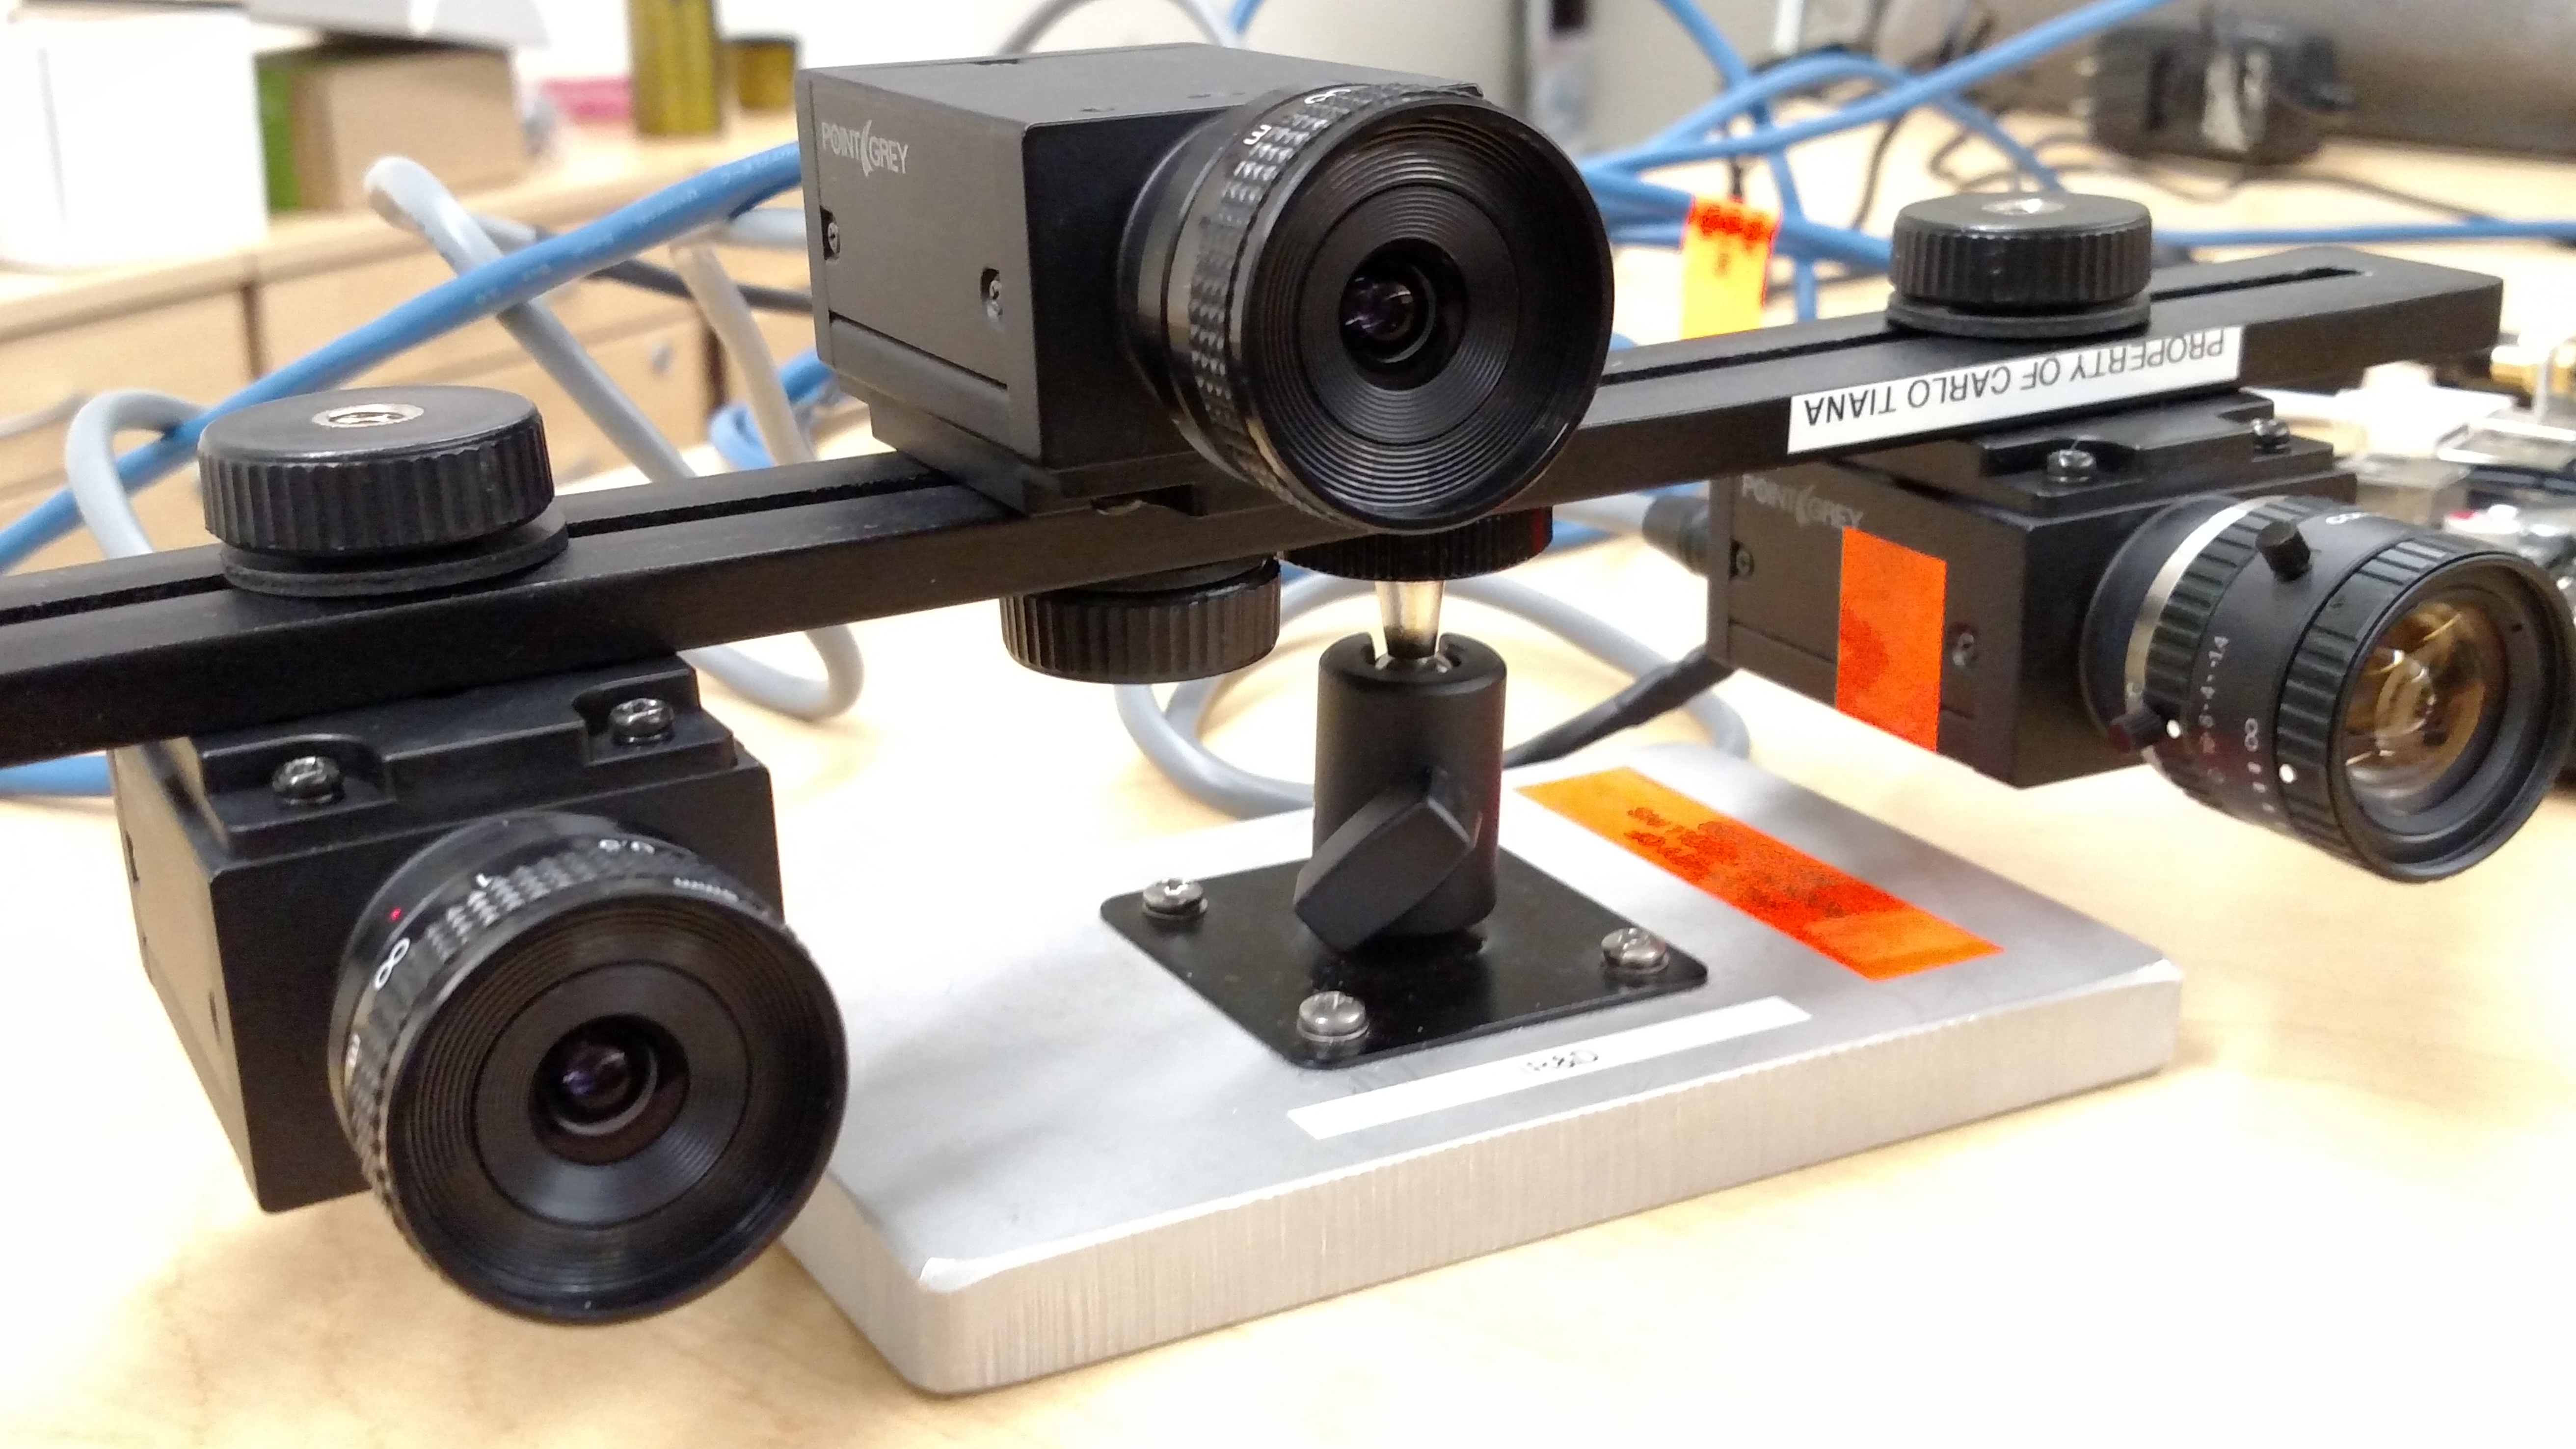
\includegraphics[width=0.6\textwidth]{IMG_20160210_131527329.jpg}
				\end{figure}
\begin{figure}[!ht]
  \caption{The Jetson TX1}
	  \centering
		    \includegraphics[width=0.6\textwidth]{rot-8.jpg}
				\end{figure}
\begin{figure}[!ht]
  \caption{The Jetson TK1}
	  \centering
		    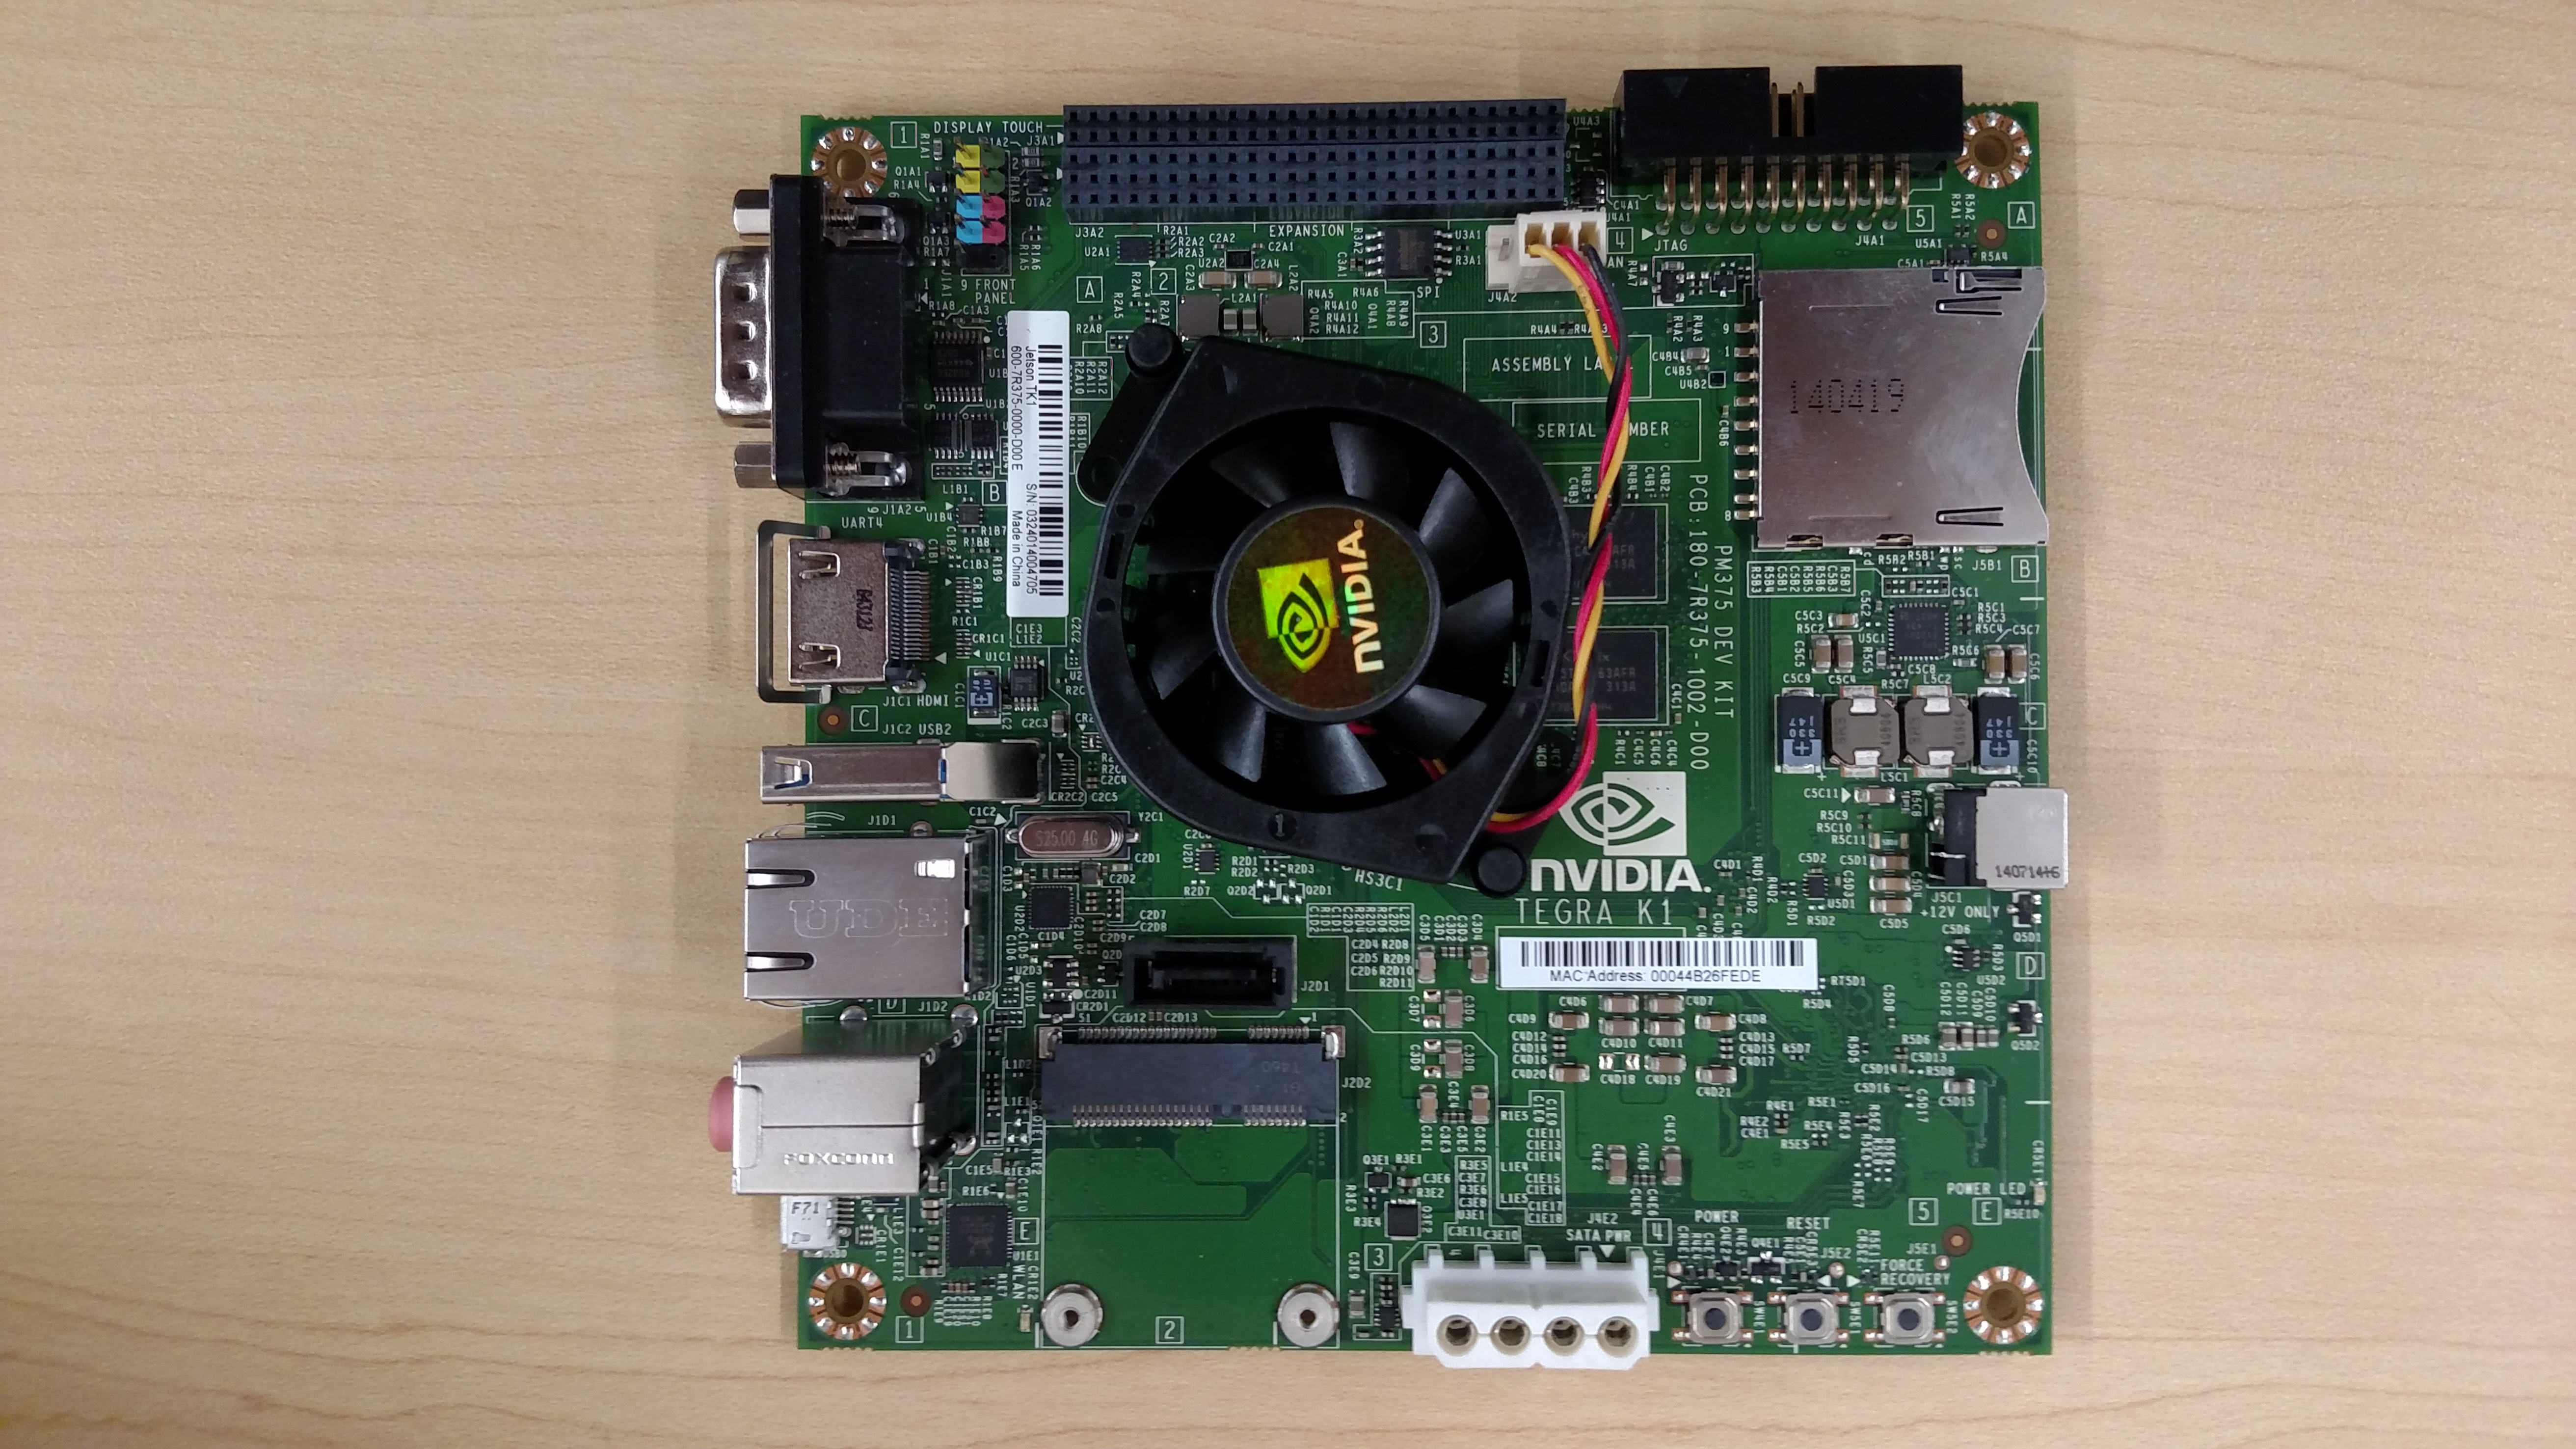
\includegraphics[width=0.6\textwidth]{rot-9.jpg}
				\end{figure}
\begin{figure}[!ht]
  \caption{The on-board camera for the TX1 }
	  \centering
		    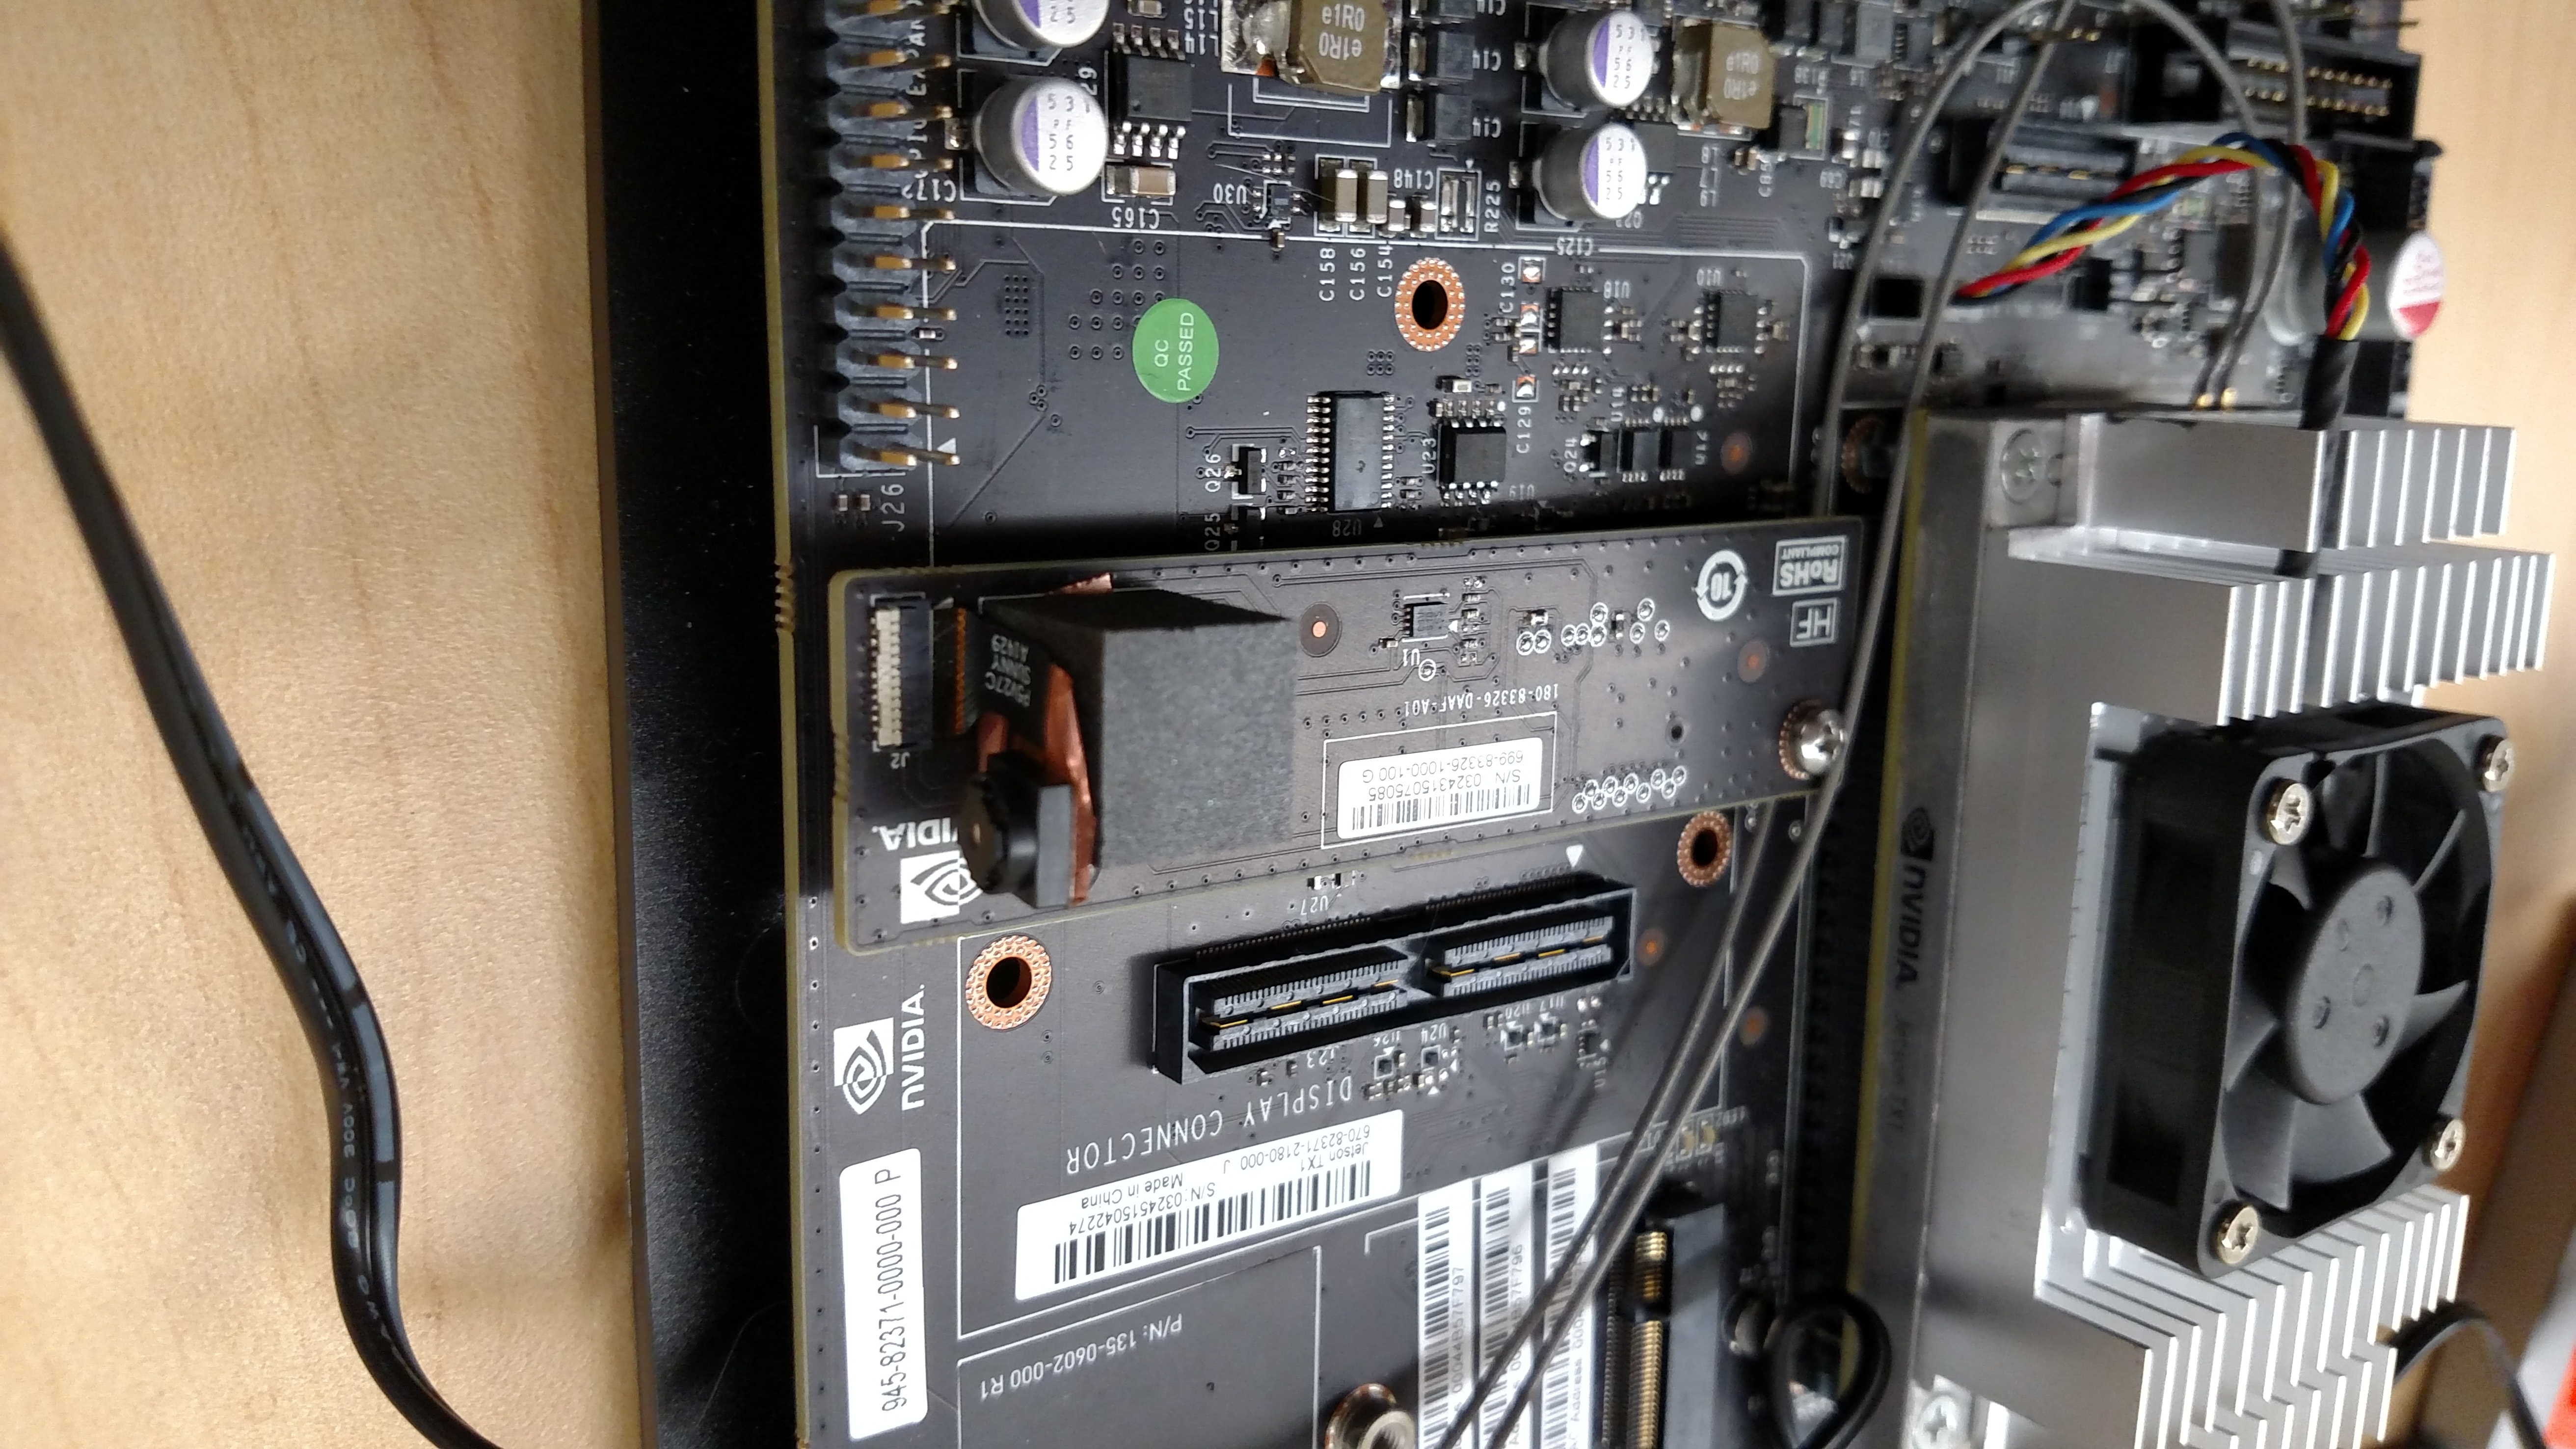
\includegraphics[width=0.6\textwidth]{rot-3.jpg}
				\end{figure}

   \subsubsection{System}
   During the wait of obtaining two more Point Grey cameras, we implemented a full modular software architecture for our vision system. Our software reads a JSON configuration file to set-up the modules. This allows for more flexibility with the use of different cameras and their software. It also gives us the ability to implement different filter modules and only apply the ones we want at a specific time. It could handle more flexibility with the use of different types of cameras only being used at specific times or for specific reasons. For example, a long range camera may only be activated when needed to find the runway from a given distance. It could then be turned on and processed when needed, but deactivated to increase the performance when it is not needed.\\ 
\par
The modular system was first able to output a static image which allowed us to demonstrate that the system was working. We then created a module to handle input from the PointGrey camera. This allowed us to interact with two of the PointGrey cameras simultaneously to get a video stream from both displayed as one video output. We have not gotten the USB PCIe card yet, so we cannot actually implement dual cameras over USB 3.0, but we are able to run one on USB 3.0 and the other on USB 2.0. Even though one of the cameras was being run with USB 2.0, we were still able to capture decent frame rate and have met our required latency goals. Further progress will require some fine tuning of the video capabilities.
   
   \section{Problems That Impeded Progress}
   \subsection{Jetson TX1 Kernel Recompile}
   We found that the Jetson TK1's operating system had to be recompiled in order to grab full 2048x2048 pixel images from the camera. Without the recompiled kernel we were able to grab images at a lower resolution using the FlyCapture API, but we needed to obtain the higher resolution to match our requirement of 1080 pixels at 30 frames per second. We had to recompile the TK1 kernel with a special version of Linux4Tegra, named "Grinch," to get the output from the USB 3.0 PointGrey camera. The recompile proved to be a difficult task and we still have some connection and display issues with the video stream. Despite these setbacks, we were able to get some video output.	
   
   \subsection{Jetson TX1 Manufacture Error}
   Development on the TX1 began slowly as we found that our first TX1 had a manufacturing problem, preventing it from connecting to wifi and causing unacceptable system lag. We notified our instructor who gave us another board that also turned out to be defective in the same way. We then had to return the TX1 we currently had, and order a new board. In the meantime we were working with the TK1, until the new fully functional TX1 arrived. When it arrived and had been tested to detect that the manufacturer error wasn't present, we were finally able to switch development from the TK1 to the TX1.
   
   \subsection{Jetson TX1 and PointGrey Camera Compatibility}
   Once we were able to interact with the USB 3.0 PointGrey camera and the Jetson TX1, we ran into the issue of getting the TX1 to register the camera and to display an image. We were finally able to get a video output from the PointGrey camera after realizing we were missing two big elements. To fix the issue, we needed to recompile the Linux kernel to increase the USB buffer size to accommodate for higher resolution image capturing from the camera, and acquired the proper camera software needed from PointGrey directly to interface between the proprietary camera API and OpenCV.
   
   \section{Preliminary Results}
   Our project requirements specification describes specific latency, frame rate, and resolution requirements in order for our system to be useful. Our end-to-end latency requirement is that it should take less than 100ms to capture video from the camera, process it, and display the outputs. Additionally, we are required to process a minimum of 30 frames per second at 1080p resolution. Our goal is to perform as much image processing as we can while maintaining these performance metrics.\\
\par
In order to measure the latency of our application, our software contains a detailed, built-in performance logging system. Each component of the software is separated into polymorphic, class-based HawkEye modules. Each individual module measures execution time including the time it takes to transfer the results to the next module. The overall latency for each frame is determined by the time it takes for all modules to finish executing from input to output, counted as the sum of the longest path. It is important to measure each individual module's latency as well as the overall latency because not all cameras are going to be subjected to the same filtering algorithms, and the additional information will enable us to predict the outcome latency based on the set of modules used. In order to measure the frame rate, we simply count the number of frames processed in a second.\\
\par
Our goal is to support independent image processing of three separate inputs. Rockwell Collins has given us some challenges outside of our requirements which we will try to implement. We have multiple types of cameras with different lenses: two standard RGB cameras and one NIR (Near infrared) camera. The IR camera will be used to identify high intensity point lights, which we will then overlay onto the processed input from one of the RGB cameras. In the industry, this would be used to identify runway lights for landing aircraft. The third camera would provide a more focused look at the target. The first performance benchmark we need to determine if this is even possible with our hardware, is to simply get three simultaneous camera feeds running at the full 30 frame per second.\\

\begin{center}
	\begin{tabular} { | l | c | c | c | }
	\hline
	\multicolumn{ 4 } { | c | } { Frame Rate} \\
	\hline
	 	      & One Camera      & Two Cameras        & Three Cameras \\ \hline
	USB 3.0 &	 37 FPS average &          		           &  \\ \hline
	USB 2.0 & 11 FPS average & 10 FPS consistent & 6 FPS \\
	\hline
	\end{tabular}
\end{center}

\par

\begin{center}
	\begin{tabular} { | l | c | c | c | }
	\hline
	\multicolumn{ 4 } { | c | } {Total Latency} \\
	\hline
	 	      & One Camera & Two Cameras & Three Cameras \\ \hline
	USB 3.0 &	 16-30 ms       &          	       &  \\ \hline
	USB 2.0 & 26-45 ms       & 38-56 ms        & 42-67 ms \\
	\hline
	\end{tabular}
\end{center}

\par
Note: One-camera usb 2.0 results are shown for comparison purposes.\\
\par
Our initial results are promising, with a single camera on USB 3.0 meeting our requirements for both FPS and latency. However, due to having only a single USB 3.0 port, our current multi-camera frame rate is much lower than the required specification. Our application is multithreaded and should not suffer full delays from additional cameras, but due to having two of the cameras using a single USB 2.0 port the delay scales linearly with each additional camera. Once we get our USB 3.0 expansion card, we should be able to significantly increase the frame rate and reduce the latency to approximately the one-camera, USB 3.0 level.\\
\par
An additional source of latency is the output windows. Currently we are running three separate windows for the three separate cameras, however to view all three at once, they must be scaled down (as currently we are running the inputs at 1080p or higher resolution). This is a processing intensive action, and can take up to 15ms to complete. Our final version is planned to combine multiple inputs and overlay them onto each other, so this operation will not have to be performed multiple times. 
  
  \subsection{Implications of Preliminary Results}
  Our preliminary results leave us with plenty of leeway as far as latency goes. We having taken only about one-fourth of the maximum total latency, however our frame rate is less than optimal. In order to increase our frame rate, we will improve our modular system to function as a buffered, pipelined system that can begin processing a frame while the previous frame is still being processed. We can do this because our latency is well below the required level, and our CPU usage is not yet at its peak. If we can begin loading a new frame while the previous frame is being processed, we will be able to maximize our usage of the USB 3.0 connection to copy new frames into memory. This is currently the slowest process and also provides the most room for improvement, as we are not yet even close to the maximum USB bandwidth. We hope to be able to maintain the same 16-25 ms latency while processing multiple frames from each camera at the same time, though if the latency increases even by doubling we will still be well within our maximum latency limit. We have already tested and seen that performing the basic operation of a colorspace conversion on a frame (which requires operations to be done on every single pixel) adds less than 2ms of latency, so we believe that we will still be able to do quite a bit of image processing within our 100ms time budget.
  
  \section{What is left to do}
  \subsection{Beta Stage}
   Since this is our alpha release, we do not have everything completed. The beta stage should be a lot more functional then our current Alpha stage. Although our alpha stage already has at least stub functionality for all the criteria we defined in our requirements document, the beta stage will improve on this and will have implemented working code for these stub functions. Some of the functions that are lacking in the alpha version, but will be completed in the beta version are:\\
   	\begin{itemize}
		\item Perform filters and video operations to test the Jetson's GPU.
		\item Improve frame rate and latency of video stream, or determine that the frame rate will never be acceptable for our criteria.
		\item Combine the streams in some logical way to demonstrate the Jetson's ability to process multiple video streams.
		\item Make the program multi-threaded to increase performance for multiple cameras.
		\item The program should be a viable example as to how to implement the same program on other similar single board computers\\
	\end{itemize}
	
	\subsection{Stretch Goals}
	If time permits, we should have the ability to implement other functions. We have planned some of these out and are considering them as stretch goals. Some of these we have already or are close to meeting:\\
	\begin{itemize}
		\item Support a third camera over USB3.
		\item Display our video feed on more than one monitor.
		\item Perform an object tracking filter.
		\item Display video operation metrics on screen. We currently log these to a file, but it would be easier to demonstrate the capabilities of the SBC if we displayed these on the video stream.
		\item Compare the Jetson with different single board computers. This would mean re-implementing our code on different platforms and comparing their processing speed and hardware capabilities.\\
	\end{itemize}
	
   \section{Interesting Piece of Code}
   The core of our program is the modular video processing pipeline. This polymorphic object-oriented system allows us to easily implement new video processing algorithms, support for different types of input devices, and new methods of outputting results. It is also responsible for measuring performance of each individual component.\\
\par
Each module is defined in its own class, which is a child class of HawkEye\_Module. Each module has two required parts, the constructor and the run() command, as well as an existing setup() command which can be overloaded as needed.\\
   \begin{lstlisting}
   	class MyModule: public HawkEye_Module{
	public:
		MyModule(){
			numinputs = 2;
			numoutputs=1;
			setup();
		}  
   \end{lstlisting}
 \par
   The initializer MUST set the number of inputs and outputs. This is extremely important because the setup() function creates the appropriate buffers and sets some internal variables needed by the module class to determine when the needed inputs have been satisfied (and thus when to execute).\\
   \begin{lstlisting}
   	void run(){
		*outputs[0] = *inputs[0]/2 + *inputs[1]/2;
	}
   \end{lstlisting}
 \par
   This is an example of what a simple module might do. The HawkEye\_Module class defines two arrays of pointers to OpenCV Mat objects, which are a kind of smart matrix/image object. This code would take two images and combine them together by a simple averaging method. OpenCV allows mass mathematical operations to be performed on all elements of a matrix, and allows adding two identically sized matrices together via simple operations as shown above. Other algorithms may require more complex operations, but this shows how simple an implementation can really be.\\
\par
Once such a module is defined, it can then be added to the parser. Currently this is a hardcoded list of module names which checks an input type name string against the predefined types and creates the associated module, however we have plans to implement a dynamically-loaded module system that allows adding new modules automatically via a dynamically linked library. After the module is added to the parser, instances can then be created in the JSON configuration file. In order to create an instance, an entry is added to the ''modules'' section of the config file.\\   
\par
A JSON configuration for our program consists of three sections: The ''modules'' section, which defines named instances of HawkEye\_Modules, the ''start'' section, which tells the program to start a camera or input, and the connections section, which defines where the output(s) from each module goes to (as a module could have multiple outputs, and some modules require multiple inputs).\\
   \begin{lstlisting}
   	{
		''modules'':{
			''MyModule_instance'':''MyModule'',
			''inputModule'':''camera'',
			''outputModule'':''basicOutput''
		},
		''start'':''inputModule'',
		''inputModule'':{TX1
			''output0'':''MyModule_instance0''
		},
		''MyModule_instance'':{
			''output0'':''outputModule0''
		}
	}
   \end{lstlisting}
 \par 
   In this example, we define two camera inputs, a combination algorithm module (as defined above in the previous code example), and an output window module. The start section tells the program that it needs to run both camera inputs, which it does separately. The code immediately after the start section tells the program to connect output 0 of inputModule1 to input 0 of MyModule\_instance, output 0 of inputModule2 to input 1 of MyModule\_instance, and the output of MyModule\_instance to the display module. When the program is executed, it will capture input from both cameras, combine it using MyModule, and then display it to a window. This configuration system makes it easy to implement complex networks of algorithm modules, and makes it so that any reconfiguration of the modules does not require a recompile of the software. This also defines the names used by the logger, in this case inputModule1, inputModule2, MyModule\_instance, and outputModule. These names can be anything the user decides to define, as long as they are consistent.

\begin{figure}[!ht]
  \caption{Video output from the TX1 using a PointGrey camera with an EVS-3000 lens attached}
	  \centering
		    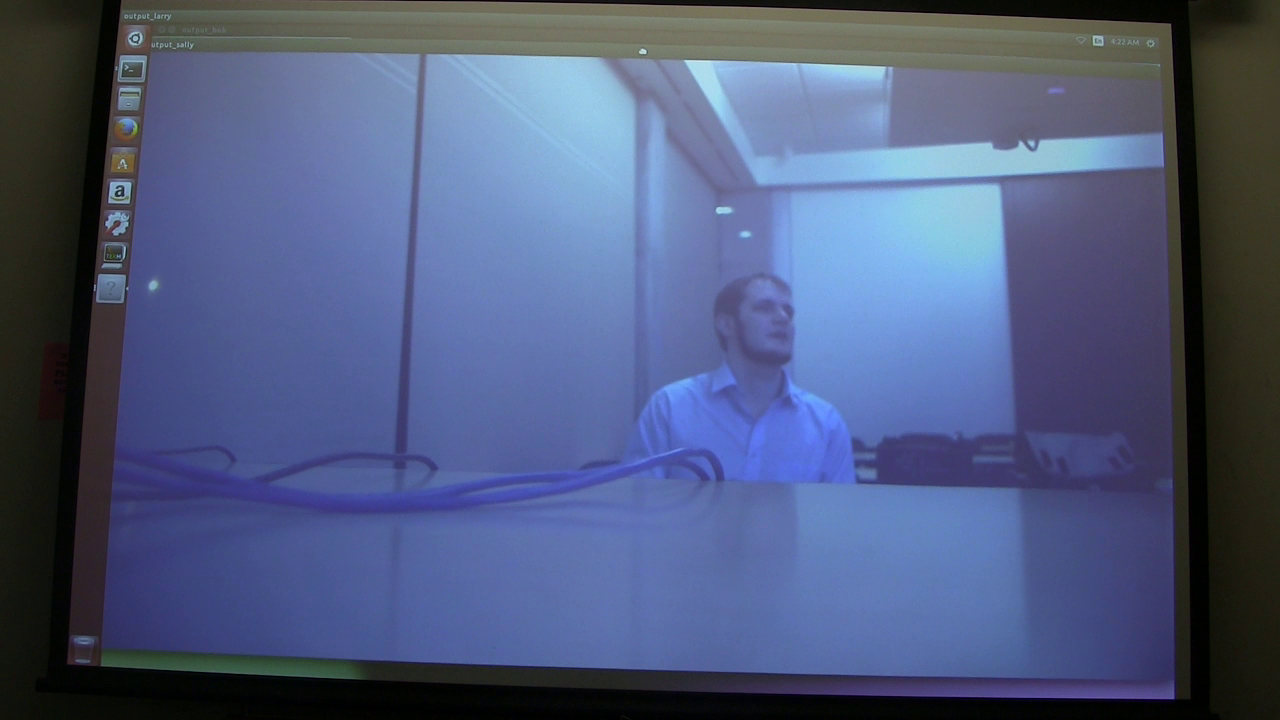
\includegraphics[width=0.6\textwidth]{vlcsnap-2016-02-11-17h42m53s150.png}
				\end{figure}
\begin{figure}[!ht]
  \caption{Video output from the TX1 using a PointGrey camera with a LS-TP-08 lens attached}
	  \centering
		    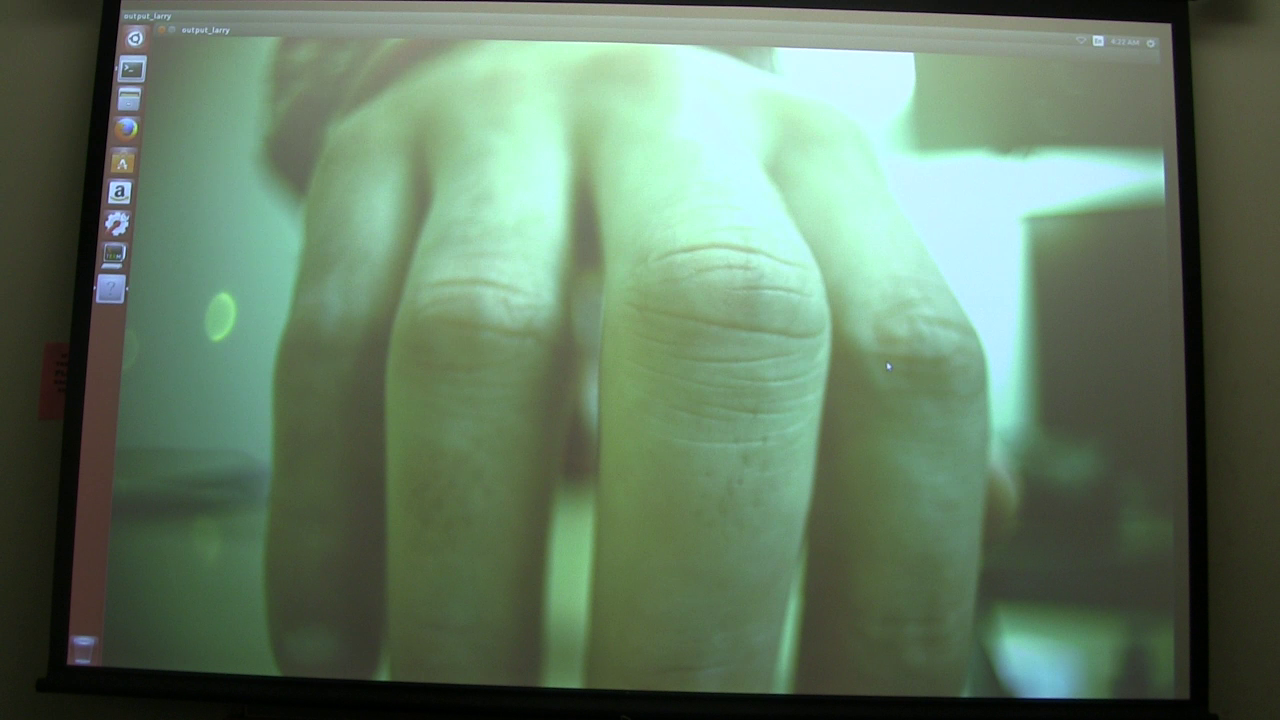
\includegraphics[width=0.6\textwidth]{vlcsnap-2016-02-11-17h42m30s486.png}
				\end{figure}

   \end{document}
